\documentclass[tikz,border=2pt]{standalone}
\usepackage{amsmath}
\usepackage{pgfplots}
\pgfplotsset{compat=1.18}

\begin{document}
% f(x)=1/x on (0,1]: for the same ε, the δ that works far from 0 (wide window) fails near 0,
% where the graph is steep and a much narrower window is needed — not uniformly continuous.
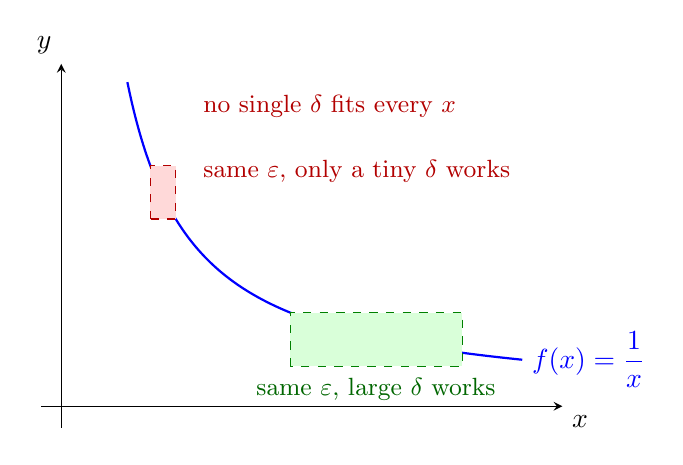
\begin{tikzpicture}
	\begin{axis}[
		axis lines=middle,
		xmin=-0.05, xmax=1.25,
		ymin=-0.4, ymax=6.4,
		xtick=\empty, ytick=\empty,
		xlabel={$x$}, ylabel={$y$},
		xlabel style={below right}, ylabel style={above left},
		samples=300, smooth, clip=false,
		width=8.2cm, height=6.2cm
		]
		\addplot[thick, blue, domain=0.165:1.15] {1/x};
		% window near x=0.8: epsilon = 0.5 around 1.25 -> x in [0.571, 1.0]: wide delta
		\fill[green!15] (axis cs:0.571,0.75) rectangle (axis cs:1.0,1.75);
		\draw[green!50!black, dashed] (axis cs:0.571,0.75) rectangle (axis cs:1.0,1.75);
		\node[green!40!black, anchor=north, font=\small] at (axis cs:0.785,0.7) {same $\varepsilon$, large $\delta$ works};
		% window near x=0.25: epsilon = 0.5 around 4 -> x in [0.222, 0.2857]: narrow delta
		\fill[red!15] (axis cs:0.222,3.5) rectangle (axis cs:0.2857,4.5);
		\draw[red!70!black, dashed] (axis cs:0.222,3.5) rectangle (axis cs:0.2857,4.5);
		\node[red!70!black, anchor=west, font=\small] at (axis cs:0.33,4.4) {same $\varepsilon$, only a tiny $\delta$ works};
		\node[red!70!black, anchor=west, font=\small] at (axis cs:0.33,5.6) {no single $\delta$ fits every $x$};
		\node[blue, anchor=west] at (axis cs:1.15,0.87) {$f(x)=\dfrac1x$};
	\end{axis}
\end{tikzpicture}
\end{document}
